\label{sec:intro}

\begin{center}
    \centering
    \noindent
    \textit{The story so far:
    In the beginning the Universe was created.
    This has made a lot of people very angry and been widely regarded as a bad move.
    }
    \vskip0.2\baselineskip
    - Douglas Adams, The Restaurant at the End of the Universe
\end{center}

\vskip0.5\baselineskip

\begin{figure}[h!]
    \centering
    \captionsetup{justification=centering}
    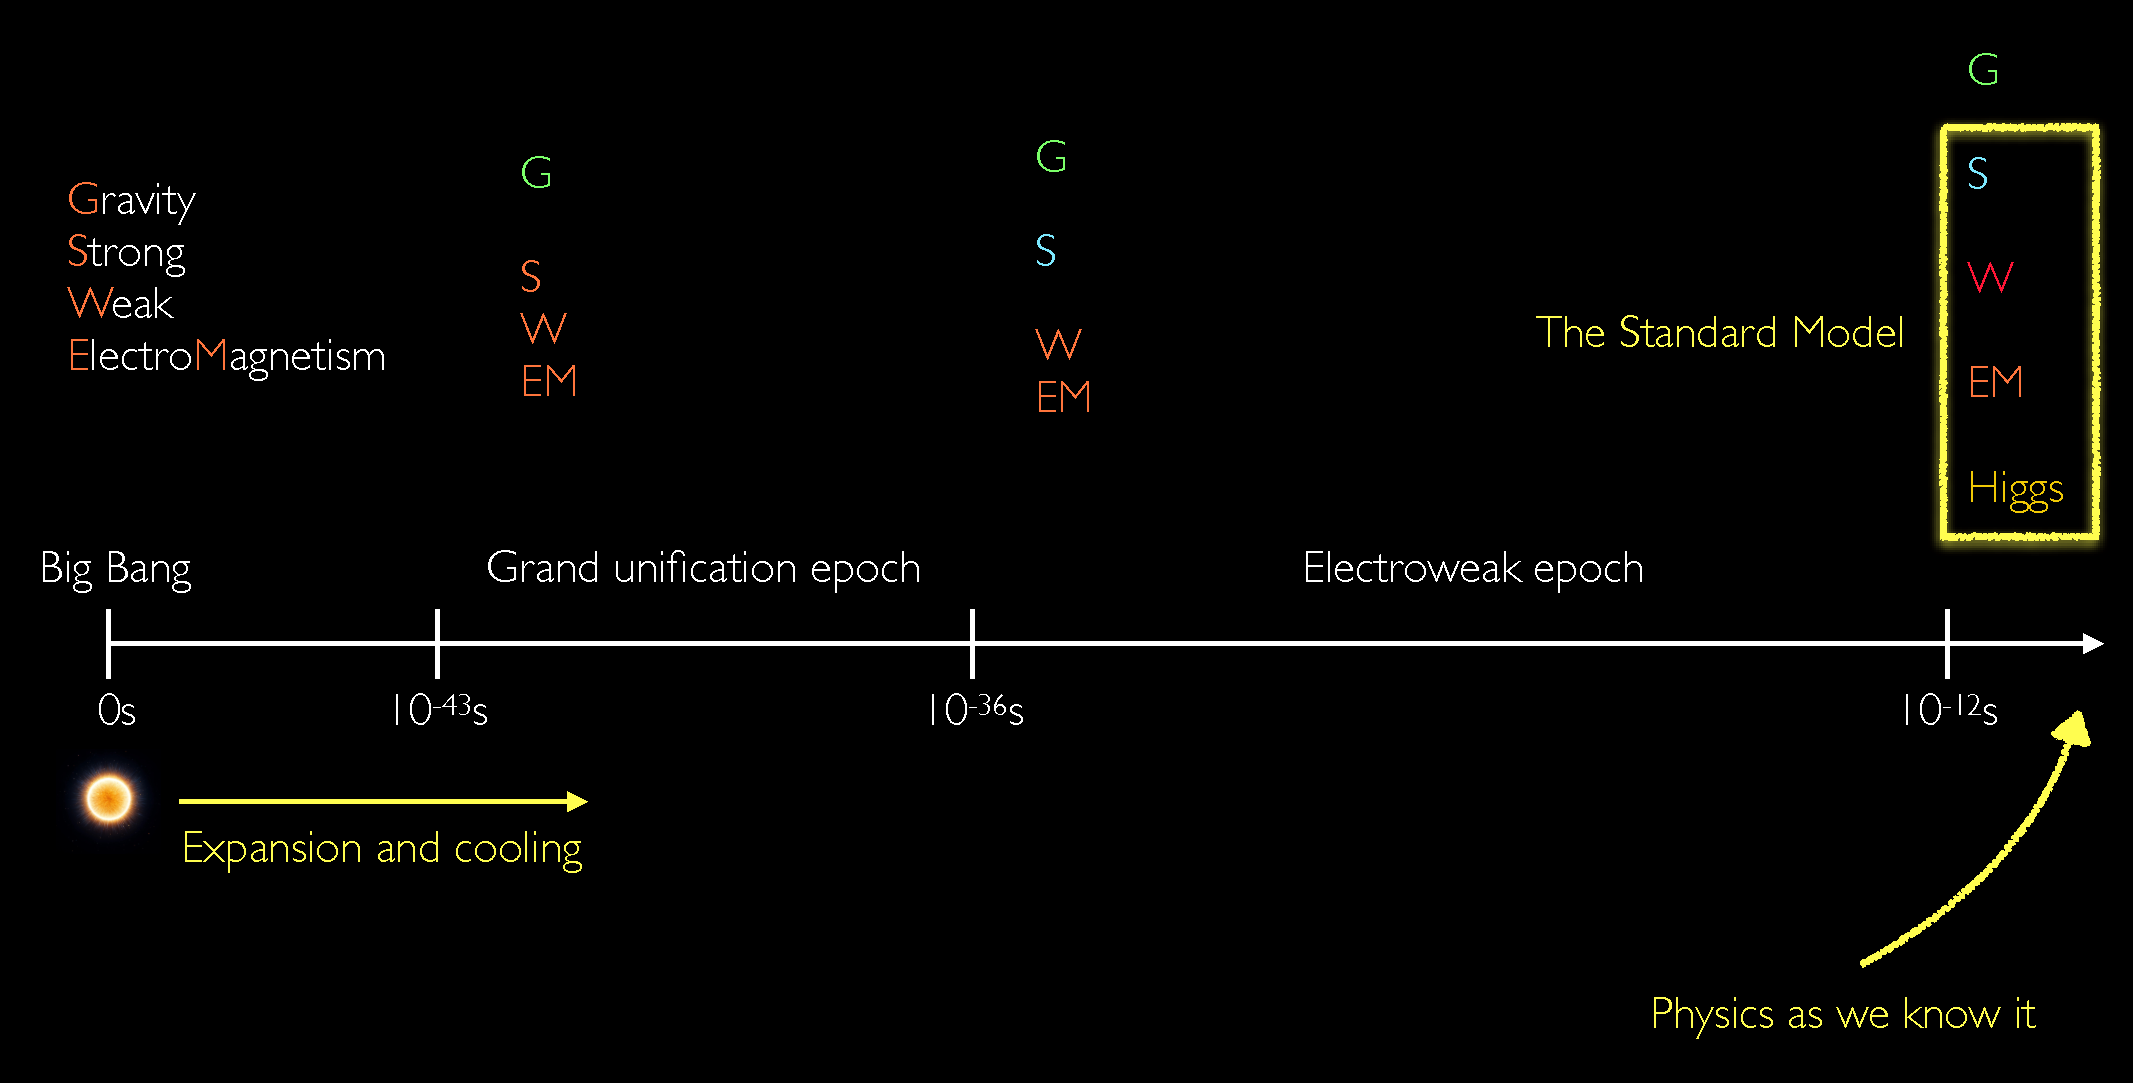
\includegraphics[width=\textwidth]{figures/00-Intro/universe_timeline.pdf}
    \caption{The timeline and evolution of forces in the early universe.}
    \label{fig:00_timeline}
\end{figure}

The universe started with a bang.
A massive burst of energy, temperature, and pressure, with all four fundamental forces --- electromagnetism, nuclear weak, nuclear strong, and gravity --- as one.
Immediately after, the universe expanded and cooled, and after about $10^{-43}$ seconds, gravity parted ways.
$10^{-36}$s later, the strong force separated as well and finally, by around $10^{-12}$s, so did the weak and electromagnetic forces,``turning on'' the Higgs field in the process and leaving us with the fundamental forces and laws of physics as we know them today (Figure~\ref{fig:00_timeline}).

Electromagnetism, the nuclear weak and strong forces, the Higgs field, and all known elementary particles can be elegantly described by the standard model (SM) of particle physics.
Over the last 60 years, it has proven a monumentally successful theory, both explaining and predicting physical phenomena up to energies produced naturally only within a nanosecond of the Big Bang.
These include the prediction of the Higgs boson 50 years before its discovery, explanations for radioactive decay and the binding of atomic nuclei, and the unification of the electromagnetic and weak forces.
However, despite its triumphs, there remain fundamental mysteries that the SM cannot explain.

The most glaring of these is its reconciliation, or lack thereof, with gravity, for which a quantum, SM-compatible theory has proven elusive.
There is also abundant cosmological evidence of ``dark'' matter and energy, constituting 95\% of the universe and yet finding no justification from the SM.
Other subtle mysteries include the inconsistency between the matter-antimatter \textit{a}symmetry  we observe and the symmetry the SM predicts, the mechanism for neutrino masses, and the origin of flavor.

The work in this dissertation is motivated by the strong possibility of many of the answers being tied to the Higgs boson.
It is our newest discovered and least understood elementary particle, and the unique nature of the Higgs field and its interactions leaves open vast potential for intriguing new physics in this sector.
As electroweak symmetry breaking, i.e., the separation of the weak and electromagnetic forces, is intimately connected to a phase transition of the Higgs field, many theories naturally link this transition with the breaking of the matter-antimatter~\cite{Morrissey_2012} and flavor symmetries~\cite{BAZZOCCHI2005372} as well.
The Higgs boson may also be the connection between the SM and the dark sector~\cite{sym13122406}, while the ``Higgs-Saw''~\cite{Krauss:2013oea} mechanism is a promising explanation for dark energy.
% seesaw~\cite{10.1143/PTP.64.1103}

Predictions of these theories include new, rare, Higgs-like particles and/or minute deviations to the interactions of the Higgs boson from the SM.
However, as many of the phenomena therein would have occurred during the electroweak epoch or earlier (see Figure~\ref{fig:00_timeline}), these effects would manifest only at the highest energies, comparable to that of $<1$ps after the Big Bang.
This dissertation presents two complementary efforts to probe such effects, by (1) searching for new, highly energetic Higgs bosons, and (2) measuring Higgs interactions uniquely sensitive to new, high energy physics.

We do so using the Large Hadron Collider (LHC) at CERN.
The LHC accelerates and collides extremely high-speed protons, producing energies comparable to the early universe just 10ps after the Big Bang.
We observe these collisions with the Compact Muon Solenoid (CMS) experiment, one of four massive detectors at the LHC, and one of the two that discovered the Higgs boson in 2012.
Crucially, we emphasize that, with the exponentially increasing rate of collisions and data at the LHC, the CMS experiment is entering an era of unprecedented potential for scientific discovery.

To fully realize this, however, and maximize the impact of our new data, significant computational innovation is required.
To this end, we also present in this dissertation several novel AI techniques to identify high energy Higgs bosons, accelerate simulations of the CMS detector, and complement traditional data analysis techniques with model-agnostic searches for new physics.
Particular emphasis is placed on the development of physics-informed machine learning (ML) algorithms, which uniquely leverage biases of high energy physics (HEP) data to improve their performance and robustness.
Namely, we introduce the first generative models for \textit{point-cloud} data in HEP, which respect the sparsity and high granularity of detector data, and the first anomaly detection models equivariant to Lorentz transformations.

We also describe significant efforts towards \textit{validating} such AI techniques, which is critical for them to ultimately have an impact in the field.
Specifically, we apply a novel method for calibrating ML algorithms targeting Higgs to vector boson decays, which has proven effective not only for the analyses presented in this dissertation but for the broader CMS physics program as well.
We additionally present several studies and new statistical techniques for evaluating fast simulations.
The combination of these and our new AI models has the potential to revolutionize the computing paradigm in CMS, improving the computational efficiency of our simulations by up to three orders of magnitude, and ensuring trust in their modeling of the underlying physics.


This dissertation is organized as follows.
Part~\ref{part:sm} introduces the theoretical basis for this dissertation, starting with the mathematical framework behind symmetries in physics (Chapter~\ref{sec:01_symmetries}) and of quantum field theory (Chapter~\ref{sec:01_qft}) before detailing the SM of particle physics (Chapter~\ref{sec:01_sm}).
Part~\ref{part:epp} then describes the experimental apparatus used in this dissertation: the LHC (Chapter~\ref{sec:02_lhc}) and the CMS experiment (Chapter~\ref{sec:02_cms}).
Part~\ref{part:aiml} concludes the background material with an introduction to ML in HEP (Chapter~\ref{sec:03_ml}), as well as the data analysis and statistical framework used in this dissertation (Chapter~\ref{sec:03_stats}).


Parts~\ref{part:ml4sim}---\ref{part:ml4jets} comprise the novel contributions of this dissertation.
Part~\ref{part:ml4sim} presents new methods for producing and validating fast simulations of the CMS detector using ML, which will be critical to maximizing the scientific output of the LHC in the coming decade.
These methods leverage advancements in generative modeling to develop novel, physics-informed simulation techniques that are orders of magnitude faster than traditional methods.
We also discuss new techniques for robust evaluation of such fast simulation techniques, and the outlook for their use in CMS.

Part~\ref{part:hh} then presents two novel searches to understand the high energy Higgs sector of the SM, targeting the production of Lorentz-boosted Higgs boson pairs, which decay into two beauty quarks and two vector bosons.
Such searches are critical to understanding the properties of the Higgs boson and searching for the effects of new physics at very high energies.
We discuss the analysis techniques used in these searches, particularly the use of deep transformer networks to identify Higgs-boson decays to two vector bosons for the first time, and competitive constraints achieved on new physics models and the two-Higgs-two-vector-boson coupling.

Finally, Part~\ref{part:ml4jets} outlines the development of new software to facilitate research in ML and HEP and ML techniques that respect the symmetries of the high energy collisions that we study.
Namely, we introduce the \jetnet Python package, which has proven impactful in this field, and a novel ML algorithm for searching for new physics while remaining robust to Lorentz-transformations of our data.
